\section{Utterance Embeddings}\label{sec:utt2vec}
\roger{This section still contains some redundant parts and needs to be restructured.}
\david{I did a first attempt at fixing it, but it still needs some (small) updates}

\subsection{Word Embeddings}
Neural networks for distributional semantics has gained relevant importance in the past years since the publication of the first neural network word embedding models.
One of the main reasons was the discovery that dense high-dimensional vector representations of words are able to capture semantic relations between words \cite{mikolov2013efficient}.
Figure~\ref{fig:w2v_example} shows a typical example where simple vector addition and subtraction lead to analogies such as: The vector difference between \textit{woman} and \textit{man} is the same as between \textit{aunt} and \textit{uncle}.


\begin{figure}
\centering
\begin{minipage}{.4\textwidth}
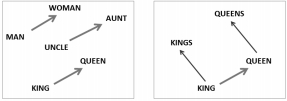
\includegraphics[width=1\textwidth]{img/w2v_example}
\caption{Word2vec semantic relations.}
\label{fig:w2v_example}
\end{minipage}
\end{figure}

In distributional semantic models, word embeddings are learned by predicting words within a context of other words.
Based on the fact that similar words occur in similar contexts, these models are capable of successfully representing words in high-dimensional vectors. 
%In order to get vector representations from utterances, we use an extension of the word embeddings neural network proposed by Mikolov\cite{mikolov2013efficient}. 

Originally, these approaches had two main architectures, know as \emph{Continuous-bag-of-words} and \emph{Skip-gram}. In the first case, the neural networks were optimized to predict the next word given its context, whereas in the latter, the context is predicted given a certain word.
Due to word co-occurrences, these models are able to effectively capture a semantic representation of the words. 
%The co-occurrence property present at the word level is no longer valid when handling phrases.

\subsection{Utterance embeddings} 
The approach from \newcite{mikolov2013efficient} is no longer feasible on a level for word sequences such as entire utterances, as the vocabulary of all possible utterances  is infinitely large, as we can construct utterances of any length.
In order to overcome this sparsity problem, a slightly different framework called \emph{paragraph2vec}\footnote{Note that despite its name, the framework is able to learn embeddings for entire word sequences of any length like sentences, paragraphs or entire documents.} for learning representations of entire word sequences has been proposed by \newcite{le2014distributed}, in which vectors are learned for a sequence from the words within the sequence.
For our case, the model thus trains utterance embeddings as well as word embeddings.
%The latter are shared for the entire model.

During training, two structures are maintained: one for words, and one for utterance representations.
The word structure is shared across the entire model, but an utterance embedding is trained for each single utterance individually.
The training task is the same as before: Given a certain window, the model is optimized to predict the missing word.
However this time, the context representation is constructed using the individual word vectors together with the utterance vector.
This training schema is called \emph{Paragraph Vector Distributed memory (PV-DM)}.  Figure~\ref{fig:p2v_arq} shows the \emph{PV-DM} architecture.

%This model makes it possible to infer vectors of fixed dimensionality for (unseen) utterances of any length.
%Its unsupervised nature permits any unannotated corpus to be used for training.

%\david{as the paragraphs above might be the complicated part of our research we should spend some time getting this as clear and readable as possible}

%\roger{The part below should be merged with the part above.}

\begin{figure}
\centering
\begin{minipage}{.3\textwidth}
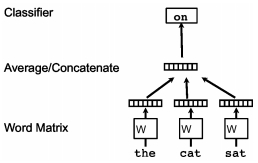
\includegraphics[width=1\textwidth]{img/par2vec_arq}
\caption{Paragraph vector PV-DM architecture.}
\label{fig:p2v_arq}
\end{minipage}
\end{figure}

Once the model is trained, it can be queried in order to get the fixed-length vector representations for each observed utterance.
It can also be used to \emph{infer} vectors for \emph{unseen} utterances.
This step is crucial to obtain the embeddings for utterances in our test dataset.

The approach presented by \newcite{le2014distributed} has two very nice advantages.
Firstly, it is completely unsupervised, and thus we can use any amount of unannotated data that is available.
Moreover, the model allows the use of pretrained word embeddings for initialization instead of initializing the parameters randomly.\footnote{Words that are not found in the pretrained model are still initialized randomly.}
This is useful if there is not enough data available to learn reliable word embeddings together with the sequence embeddings.
For our experiments, we try both methods: training word and paragraph embeddings entirely from scratch using different dialog corpora as input, as well as using the freely available pretrained word embeddings based on the \emph{Google News Corpus}\footnote{\url{https://code.google.com/p/word2vec/}} to initialize the model.
